%%%%%%%%%%%%%%%%%%%%%%%%%%%%%%%%%%%%%
\chapter{Standard Model and rare Z and Higgs decays to quarkonia}
\label{chaptertheory}

\section{Standard Model and Local Gauge Invariance}
\label{section_sm}

% The human quest for understanding the Universe, goes through taking a complex problem and break it down into smaller (simpler) ideas, that, when stacked together, gives rise to a proper explanation of a phenomenon and, in the best scenario, allows us to make predictions about unexpected or less known aspects of subject. The Standard Model (SM) embodies this idea and attempts not only to explain the Universe in fundamental process (interactions), but also in terms of fundamentals components (particles). To what it proposes to explain, the Standard Model have been proven very effective.
 
Physics understands matter and how it interacts in terms of two components: fundamentals forces and elementary particles. From the weakest to the strongest, the fundamental forces are: Gravitational, Weak, Electromagnetic and Strong. All share common characteristics like, being mediated by particles~\footnote{There is no evidence of the existence of the Graviton (force carrier associated to the gravitational force), even though, it is theorized by models that wish to comprehend gravity in a quantum perspective.}, being relevant within some effective range and have a associate a charge-like quantity (i.e. an intrinsic characteristic of the object) that defines whether or not, particles might be subjected to a specific interaction.

Along with the fundamental interactions, the Standard Model~\cite{burgess_moore_2006, oguri_qcd, Halzen:1984mc, Aitchison:2004cs} (or simply \textit{SM}) defines every existing matter in the Universe as a set of fundamental quantum objects, with properties that prescribes their interaction. Those objects are said to be fundamental since, in the context of the SM, they are the smallest possible components of matter. We shall refer to them as \textit{Fundamental Particles}. There four of those mediating particles (force carriers), gluon ($g$ - for the strong interaction), photon ($\gamma$ - for the electromagnetic interaction), Z and W (for weak interaction), all of them being vector bosons (spin 1). Besides the interaction mediators, described at Table~\ref{fundamental_forces}, the fundamental particles are divided in two groups (\textit{quarks} and \textit{leptons}), with three generations, each. These are not force carriers, but elementary particles, endowed with charge-like characteristics that allow them to interact by exchange the vector bosons. Those are the building blocks of Matter in our Universe.

Figure~\ref{sm_summary} summarizes their properties. Table~\ref{fundamental_forces} presents the relative strength and effective range, for each on of the four fundamental interactions. It is important to stress that, the gravitational force is not study subject of the Standard Model.

\begin{figure}[!htbp]
  \begin{center}
  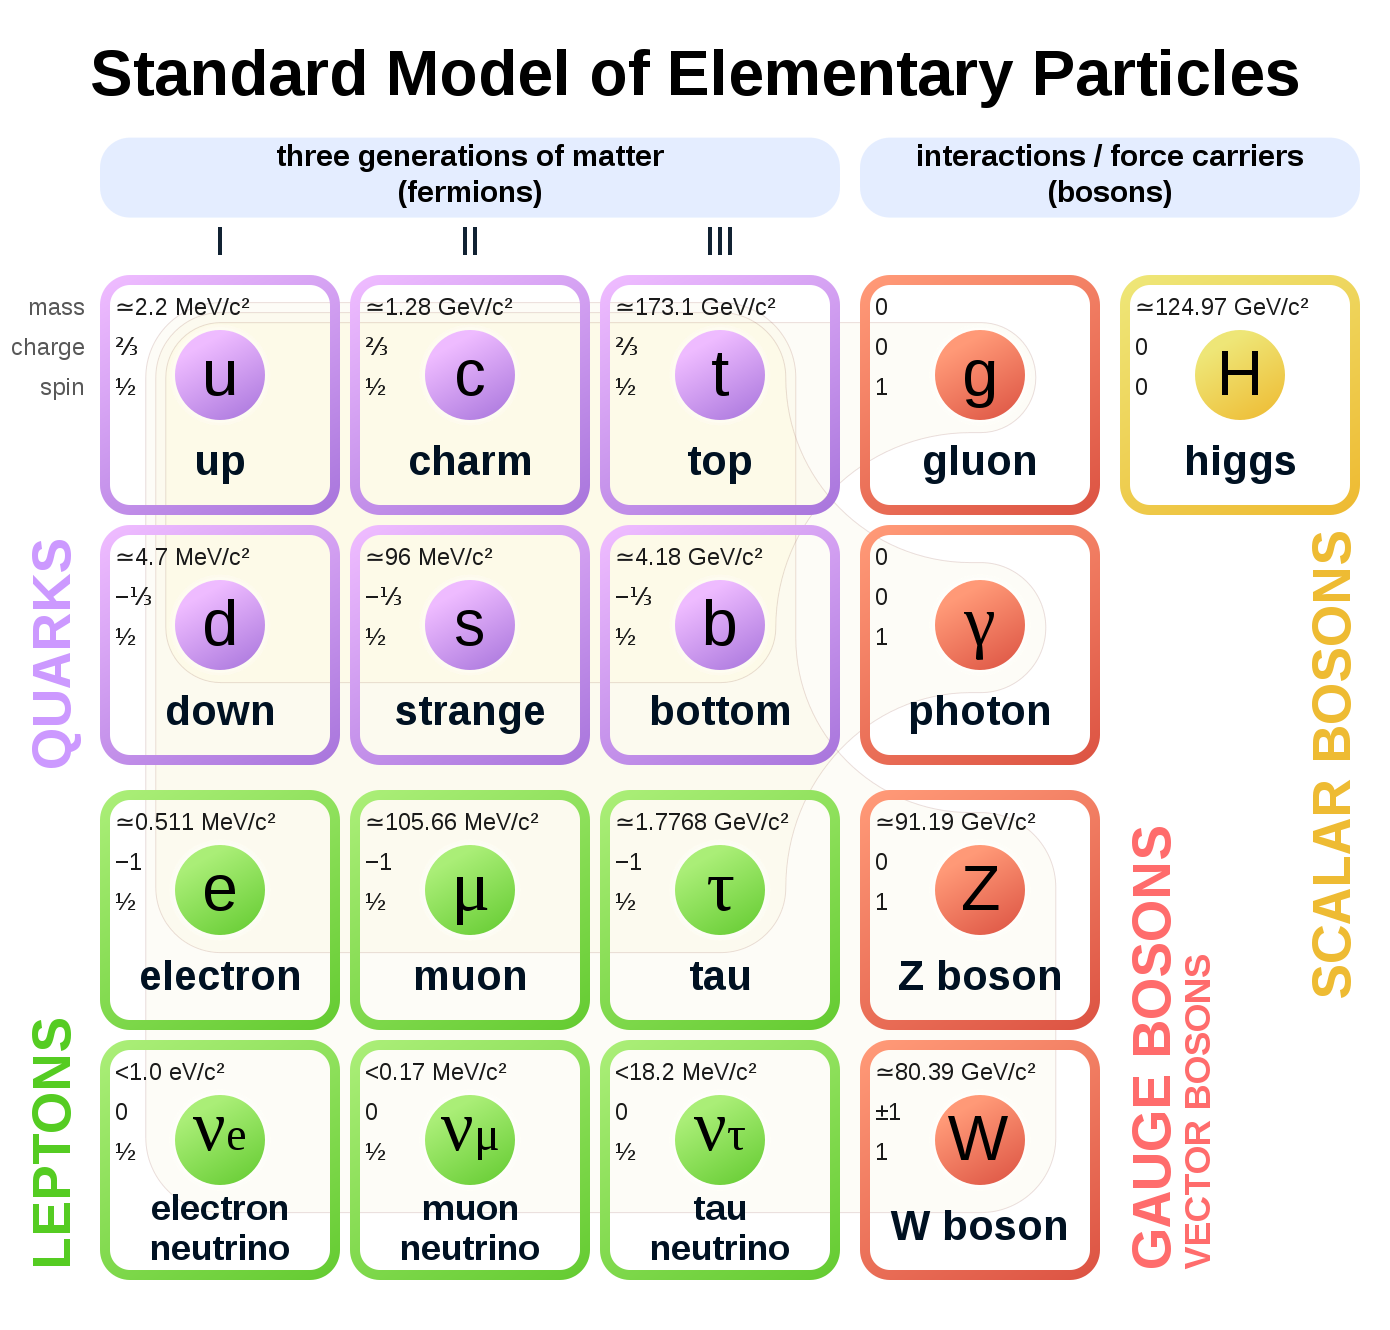
\includegraphics[width=0.6\textwidth ]{figures_and_tables/theory/sm.png}
  \end{center}\vspace*{-.5cm}
  \caption{Elementary particles of the Standard Model, with their masses charges and spin. Those particles can be divided in two classes: boson (the interaction/force carriers) and the fermions, which are divided in three generations. Source:~\cite{fig_sm_summary}.}
  \label{sm_summary}
  \end{figure}
 

\begin{table}[htp]
  \begin{center}
      \caption{Relative strength (with respect to the strong force) and effective range of action for the four fundamentals interactions.}
    \begin{tabular}{ cccc }
       & Mediator & Relative Strength & Effective Range \\ \hline
      Gravitational & Graviton & $10^{-41}$ & $\infty$ \\ 
      Weak & W and Z & $10^{-16}$ & $10^{-18}$ m \\ 
      Electromagnetic & Photon & $10^{-3}$ & $\infty$ \\ 
      Strong & Gluon & $1$ & $10^{-15}$ m\\ \hline
      \end{tabular}
  \label{fundamental_forces}
  \end{center} 
  \end{table}


There are six quarks, up and down ($u$ and $d$ - first generation), charm and strange ($c$ and $s$ - second generation), top and bottom ($t$ and $b$ - third generation), in increasing invariant mass order of the generations. Since they interact through all the three fundamental forces of the SM, they are said to possess electrical charge (for the electromagnetic interaction), flavour (for the weak interaction) and color (for the strong). Their generational counterparts, the leptons, don't interact via strong force, that is why they are said to have only flavour and electric charge. The leptons are electron and electron neutrino ($e$ and $\nu_e$ - first generation), muon and muon neutrino ($\mu$ and $\nu_{\mu}$ - second generation) and tau and tau neutrino ($\tau$ and $\nu_{\tau}$ - third generation). The neutrinos, within the SM, are massless, even though, experimental measurements have shown that they actually have mass~\cite{pdg_2020}. Neutrinos are also electrically neutral, meaning that they only interact through weak interactions.

Figure~\ref{sm_summary} also presents the Higgs Boson ($H$) which is part of the SM and shall be discussed later.

\subsection{Local Gauge Invariance}

Within the Standard Model, the theoretical basis that describe the fundamental interactions are derived from a common principle: the local gauge invariance. According to Salam and Ward~\cite{ward_salam}:

\begin{quote}
  "Our basic postulate is that it should be possible to generate strong, weak and electro-magnetic interaction terms [...], by making local gauge transformations on the kinetic-energy terms in the free Lagrangian for all particles."
\end{quote}

Taking the Quantum Electrodynamics (QED) as an example: the quantum field theory that describes the electromagnetic interactions, consider the Dirac equation, in the covariant form, for a particle with mass $m$, charge $-e$ and spin $1/2$, i.e. a electron:

\begin{equation}
    (i \gamma^\mu \partial_\mu + m)\psi(x) = 0,
    \label{dirac_equation}
\end{equation}
where $\psi(x)$ is a spinor, describing the wave-function and $\gamma^\mu$ are gamma-matrices. This equation can be obtained from the lagrangian $\mathcal{L}$~\footnote{Even though, the $\mathcal{L}$ actually represents the lagrangian density, in this document we shall refer to it as simply lagrangian.} of a free particle, in the form of 

\begin{equation}
    \mathcal{L_{\text{0}}} = i\bar{\psi}(x)\gamma^\mu\partial_\mu\psi(x)-m\bar{\psi}\psi(x),
    \label{lagrangian_free_particle}
\end{equation}
when applied to the Euler-Lagrange equation.

It is clear that, the Dirac Equation (\ref{dirac_equation}) and its lagrangian (\ref{lagrangian_free_particle}) are invariant under a global phase transformation.

\begin{equation}
    \psi(x) \rightarrow \psi'(x) = \exp{(-ie\alpha)}\psi(x),
    \label{global_phase_transformation}
\end{equation}
where is a constant (global phase shift).

The same is not true when $\alpha$ is not a constant, but actually a local phase transformation, a gauge transform.

\begin{equation}
    \psi(x) \rightarrow \psi'(x) = \exp{(-ie\alpha(x))}\psi(x)
    \label{local_phase_transformation}
\end{equation}

In this case, the derivative of $\alpha(x)$ will introduce a new term that would break the invariance. To recover it, the covariant derivative operator should be modified as follows:

\begin{equation}
    \partial_\mu \rightarrow D_\mu = \partial_\mu - ieA_\mu.
    \label{covariant_derivative_modification}
\end{equation}

This modification introduces the concept of the gauge field $A_\mu$, associated to a particle of spin 1 and zero mass, the photon. This term should transform under gauge, in the following manner:

\begin{equation}
    A_\mu \rightarrow A'_\mu = A_\mu - \partial_\mu\alpha(x).
    \label{covariant_gauge_field}
\end{equation}

Modifications \ref{covariant_derivative_modification} and \ref{covariant_gauge_field} are sufficient not only to make the free particle Dirac Equation and its lagrangian gauge transformation invariant (Equations \ref{invariant_dirac_equation} and \ref{invariant_lagrangian} ), but also it naturally gives rise to an interaction term associated to the gauge field $A_\mu$.

\begin{equation}
        (i \gamma^\mu \partial_\mu + m)\psi(x) = -e\gamma_\mu A_\mu(x) \psi(x) 
    \label{invariant_dirac_equation}
\end{equation}
\begin{equation}
    \begin{split}
        \mathcal{L} \rightarrow \mathcal{L'} &= i\bar{\psi'}(x)\gamma^\mu\ D_\mu\psi'(x)-m\bar{\psi'}\psi'(x) \\
        \mathcal{L'} &= \mathcal{L_{\text{0}}} + e\bar{\psi}(x)\gamma^\mu A_\mu \psi(x) = \mathcal{L}
    \end{split}
    \label{invariant_lagrangian}
\end{equation}

Interesting to notice that the $\mathcal{L_{\text{0}}}$, on \ref{invariant_lagrangian} term corresponds to the electron kinetic energy plus the mass contribution (the free particle lagrangian), while the second corresponds to the interaction of the electron ($\psi(x)$) and the electromagnetic field. One could add the energy contribution of the electromagnetic field itself, by adding a term like:

\begin{equation}
    \mathcal{L_{\text{EM}}} = - \frac{1}{4} F_{\mu\nu} F^{\mu\nu},
\label{lagragian_em}
\end{equation}
where:
\begin{equation}
    F_{\mu\nu} = \partial_\mu A_\nu - \partial_\nu A_\mu.
\label{f_munu_definition}
\end{equation}

It can be proven that applying \ref{f_munu_definition} on the Euler-Lagrange equations, this will give us the Maxwell's Equations for the vacuum, $\partial_{\mu} F^{\mu\nu} = 0$~\footnote{A non-vacuum covariant form of the Maxwell's Equations would be $\partial_{\mu} F^{\mu\nu} = j^{\nu}$.}. One could also expect that a field mass contribution in as below, could be introduced, as well.

\begin{equation}
    \frac{1}{2}m A_\mu A_\mu
\label{photon_mass_term}
\end{equation}

This one would break the gauge invariance, therefor we could imply that the photon should be massless.

\subsection{The Standard Model}

Taking profit of the Local Gauge Invariance as path to introduce interactions in a quantum field theory, such as for the QED, the Standard Model can be defined as 



\todo[inline]{SM as a gauge theory} 
\todo[inline]{Spontaneous Symmetry break and the Higgs Boson} 
